\documentclass[tikz,border=2pt]{standalone}
\usepackage{amsmath,amssymb}
\usepackage{tikz}
\usetikzlibrary{arrows.meta}

\begin{document}
% Scalar multiplication stretches (|c| > 1), shrinks (|c| < 1) or flips (c < 0) a vector
% along its own line.
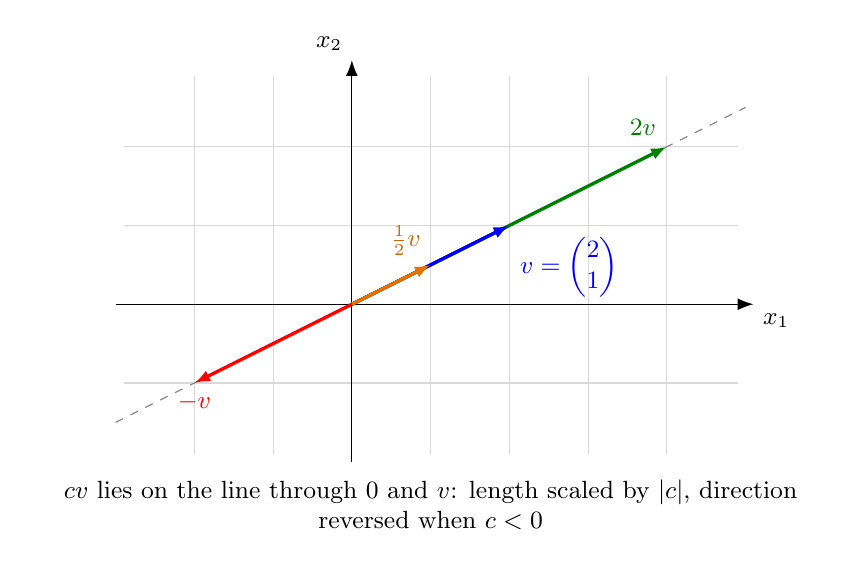
\begin{tikzpicture}[every node/.style={font=\small}, >={Latex[length=2mm]}]
	\draw[gray!30, step=1] (-2.9,-1.9) grid (4.9,2.9);
	\draw[->] (-3,0) -- (5.1,0) node[below right] {$x_1$};
	\draw[->] (0,-2) -- (0,3.1) node[above left] {$x_2$};
	\draw[gray, dashed] (-3,-1.5) -- (5,2.5);
	\draw[->, green!50!black, very thick] (0,0) -- (4,2) node[above left] {$2v$};
	\draw[->, blue, very thick] (0,0) -- (2,1) node[below right] {$v=\begin{pmatrix}2\\1\end{pmatrix}$};
	\draw[->, orange!90!black, very thick] (0,0) -- (1,0.5);
	\node[orange!80!black, above left, font=\small] at (1,0.5) {$\tfrac12v$};
	\draw[->, red, very thick] (0,0) -- (-2,-1) node[below] {$-v$};
	\node[anchor=north, align=flush center, text width=10cm] at (1,-2.1) {$cv$ lies on the line through $0$ and $v$: length scaled by $|c|$, direction reversed when $c<0$};
\end{tikzpicture}
\end{document}
